% !TEX TS-program = pdflatex
% !TEX encoding = UTF-8 Unicode

% This is a simple template for a LaTeX document using the "article" class.
% See "book", "report", "letter" for other types of document.

\documentclass[11pt]{report} % use larger type; default would be 10pt

\usepackage[utf8]{inputenc} % set input encoding (not needed with XeLaTeX)

%%% Examples of Article customizations
% These packages are optional, depending whether you want the features they provide.
% See the LaTeX Companion or other references for full information.

%%% PAGE DIMENSIONS
\usepackage{geometry} % to change the page dimensions
\geometry{a4paper} % or letterpaper (US) or a5paper or....
% \geometry{margin=2in} % for example, change the margins to 2 inches all round
% \geometry{landscape} % set up the page for landscape
%   read geometry.pdf for detailed page layout information

\usepackage{graphicx} % support the \includegraphics command and options

% \usepackage[parfill]{parskip} % Activate to begin paragraphs with an empty line rather than an indent

%%% PACKAGES
\usepackage{booktabs} % for much better looking tables
\usepackage{array} % for better arrays (eg matrices) in maths
\usepackage{paralist} % very flexible & customisable lists (eg. enumerate/itemize, etc.)
\usepackage{verbatim} % adds environment for commenting out blocks of text & for better verbatim
\usepackage{subfig} % make it possible to include more than one captioned figure/table in a single float
\usepackage{enumitem}

% These packages are all incorporated in the memoir class to one degree or another...

%%% HEADERS & FOOTERS
\usepackage{fancyhdr} % This should be set AFTER setting up the page geometry
\pagestyle{fancy} % options: empty , plain , fancy
\renewcommand{\headrulewidth}{0pt} % customise the layout...
\lhead{}\chead{}\rhead{}
\lfoot{}\cfoot{\thepage}\rfoot{}

%%% SECTION TITLE APPEARANCE
\usepackage{sectsty}
\allsectionsfont{\sffamily\mdseries\upshape} % (See the fntguide.pdf for font help)
% (This matches ConTeXt defaults)

%%% ToC (table of contents) APPEARANCE
\usepackage[nottoc,notlof,notlot]{tocbibind} % Put the bibliography in the ToC
\usepackage[titles,subfigure]{tocloft} % Alter the style of the Table of Contents
\renewcommand{\cftsecfont}{\rmfamily\mdseries\upshape}
\renewcommand{\cftsecpagefont}{\rmfamily\mdseries\upshape} % No bold!

\usepackage[hidelinks]{hyperref}
\usepackage{float}

\usepackage[italian]{babel}

\usepackage{biblatex} %Imports biblatex package
\bibliography{citations} %Import the bibliography file

\setlength{\parindent}{0cm}

\usepackage{listings}
\usepackage{color}
\definecolor{lightgray}{rgb}{.9,.9,.9}
\definecolor{darkgray}{rgb}{.4,.4,.4}
\definecolor{purple}{rgb}{0.65, 0.12, 0.82}

\lstdefinelanguage{SWRL}{
  keywords={},
  otherkeywords={^, ->},
  keywordstyle=\color{blue}\bfseries,
  identifierstyle=\color{black},
  sensitive=false,
  breakatwhitespace=true
}

\lstset{
   backgroundcolor=\color{lightgray},
   extendedchars=true,
   basicstyle=\footnotesize\ttfamily,
   showstringspaces=false,
   showspaces=false,
   numbers=none,
   tabsize=2,
   breaklines=true,
   showtabs=false,
   captionpos=b
}

\usepackage{graphicx}
\graphicspath{ {./img/} }

%%% END Article customizations

%%% The "real" document content comes below...

\title{FootOntologyPlus}
\author{
  Giacomo Leo Bertuccioli\\
  \texttt{0001136879}
  \and
  Alex Mazzotti\\
  \texttt{matricola}
}
\date{} % Activate to display a given date or no date (if empty),
         % otherwise the current date is printed 

\begin{document}
\maketitle

\newpage

\renewcommand*\contentsname{Indice}

\tableofcontents
\newpage

\chapter{Introduzione}

Footology \cite{foot} è un knowledge representation system progettato per rappresentare e organizzare le informazioni rilevanti del mondo del calcio.
L'ontologia consente di modellare i diversi aspetti e concetti del gioco, come ad esempio partite, squadre di calcio e giocatori.
L'idea dietro al progetto è quella di facilitare l'integrazione dei dati, l'interoperabilità e fornire sistemi di interrogazione avanzati per applicazioni riguardanti il calcio.

\hfill

La nostra estensione FootOntologyPlus mira ad espandere l'originale, modellando meglio alcuni dei concetti inclusi da quest'ultima o aggiungendone di nuovi.
L'entità delle nostre modifiche è discussa nei capitoli successivi.

\hfill

Il nostro progetto è stato realizzato usando l'editor \textbf{Protegé}, un programma open source per visualizzare e modificare ontologie.

\chapter{Ontologia di partenza}

\section{Informazioni di base}

Footology è disponibile su Github \cite{foot}, pubblicata dall'utente \textbf{arditb1997}, ed è un'ontologia relativamente semplice che modella gli aspetti principali del calcio.

\hfill

L'ontologia è disponibile in 3 formati diversi: \textbf{owl}, \textbf{rdf} e \textbf{ttl}.
\textbf{OWL} e \textbf{RDF} sono due linguaggi di knowledge representation, mentre il terzo, \textbf{Turtle}, è semplicemente una sintassi usata per esprimere ontologie scritte in uno dei due linguaggi precedenti in un formato testuale più facile da leggere. 

\section{Dettagli dell'ontologia}

La seguente tabella riassume i contenuti dell'ontologia:

\begin{center}
    \begin{tabular}{||c|c||}
        \hline
        Classi & \texttt{13} \\
        \hline
        Object properties & \texttt{26} \\
        \hline
        Data properties & \texttt{46} \\
        \hline
        Individui & \texttt{0} \\
        \hline
        Nodi (del grafo) & \texttt{59} \\
        \hline
        Foglie (del grafo) & \texttt{62} \\
        \hline
    \end{tabular}
\end{center}

\section{Classi dell'ontologia}

Le classi contenute nell'ontologia sono:

\begin{itemize}
    \item \texttt{Player}, che rappresenta un calciatore;
    \item \texttt{Team}, che rappresenta una squadra di calcio;
    \item \texttt{Match}, una partita di calcio;
    \item \texttt{PerformanceStats}, statistiche riguardanti un calciatore in una partita o all'intera partita;
    \item \texttt{Tournament}, un torneo di calcio, che ha come sottoclassi \texttt{KnockOutTournament}, un torneo piramidale ad eliminazione diretta, e \texttt{League}, un torneo in cui ogni squadra affronta tutte le altre e accumula punti in base al risultato delle partite;
    \item \texttt{Stadium}, uno stadio in cui si giocano le partite;
    \item \texttt{Coach}, un allenatore;
    \item \texttt{Referee}, un arbitro;
    \item \texttt{Position}, la posizione di un giocatore in partita;
    \item \texttt{Trophy}, un trofeo vinto da una squadra;
    \item \texttt{Award}, un premio vinto da un giocatore.
\end{itemize}

\section{Proprietà importanti}

Le proprietà più importanti nell'ontologia sono:

\begin{itemize}
    \item \texttt{playsFor}, che collega un giocatore a una squadra in cui gioca;
    \item \texttt{participatesIn}, che collega un giocatore a una partita a cui partecipa;
    \item \texttt{competesIn}, che collega una squadra a una partita in cui è coinvolta;
    \item \texttt{partOf}, che collega una squadra ad un torneo a cui partecipa;
    \item \texttt{hasStats} e \texttt{hasPerformanceStats}, che collegano rispettivamente un giocatore e una partita a delle statistiche;
    \item \texttt{hosts}, che collega uno stadio ad una partita;
    \item \texttt{officiates}, che collega un arbitro ad una partita;
    \item \texttt{manages}, che collega un allenatore ad una squadra.
\end{itemize}
    
\begin{figure}[H]
    \begin{center}
        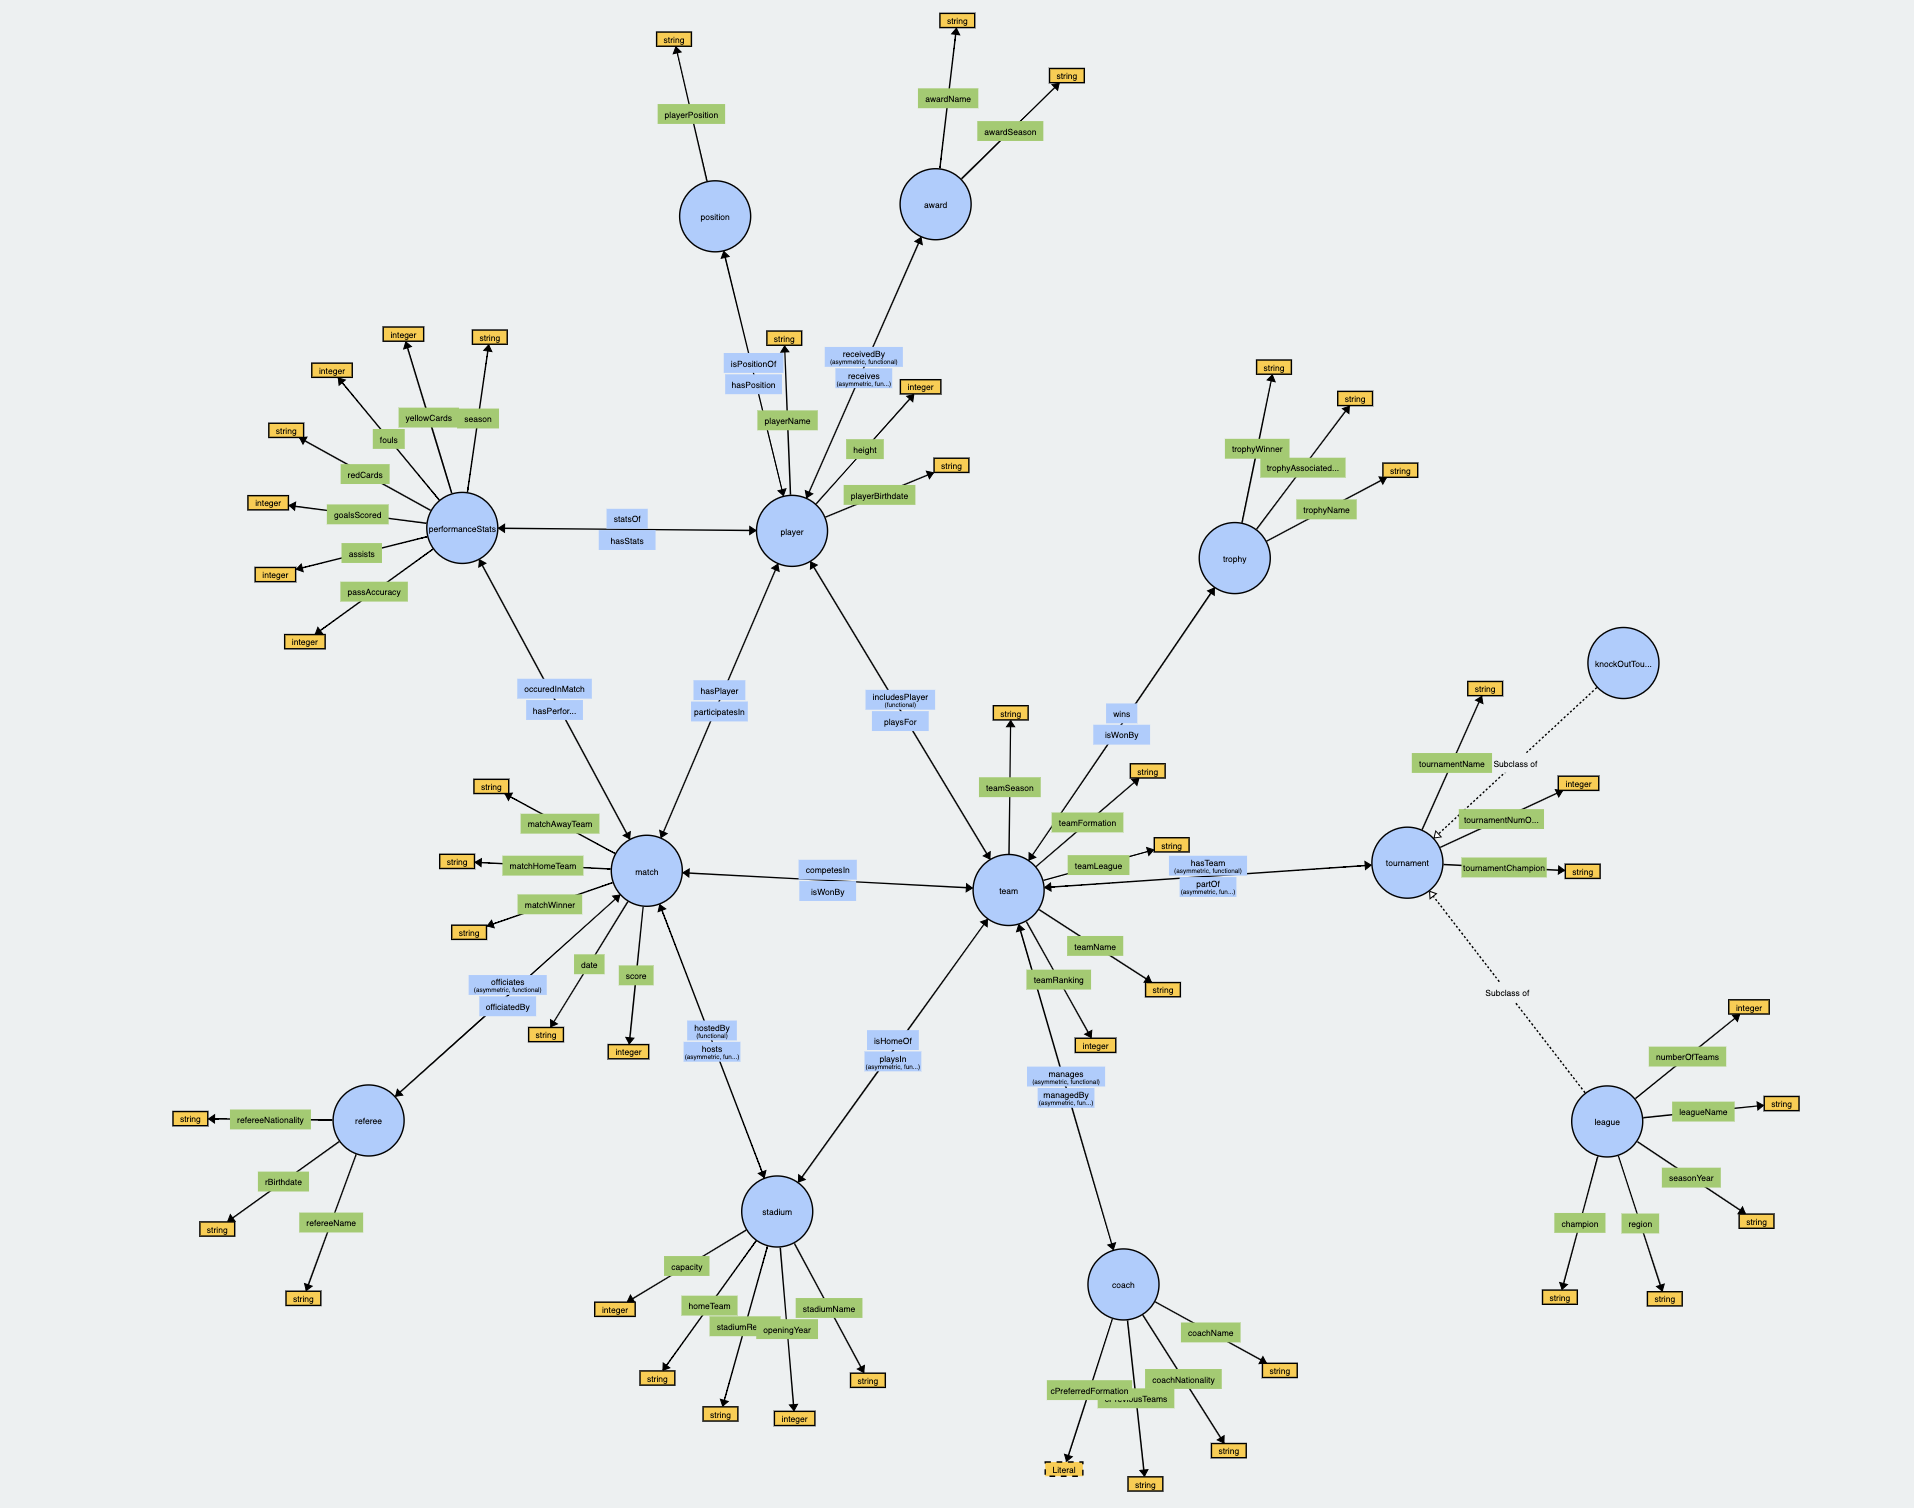
\includegraphics[width=0.85\textwidth]{footology_2.1.png}
    \end{center}
    \caption{Grafico dell'ontologia, realizzat0 con WebVOWL \cite{webvowl,foot}.}
\end{figure}
\begin{figure}[H]
    \begin{center}
        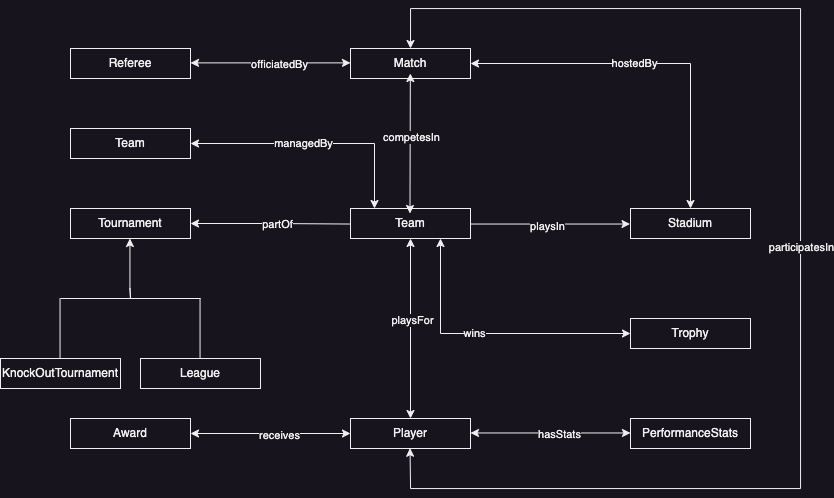
\includegraphics[width=0.85\textwidth]{footology_v2.1_schema.png}
    \end{center}
    \caption{Schema dell'ontologia, realizzato con Draw.io \cite{drawio, foot}.}
\end{figure}
    
\section{Ontologie incluse}

Per realizzare l'ontologia sono stati utilizzati:

\begin{itemize}
    \item \textbf{RDF} (\textbf{Resource Description Language}), un modello per la rappresentazione di dati (e metadati), avente una struttura graph-based nella quale essi sono scritti sotto forma di triple soggetto-predicato-oggetto;
    \item \textbf{RDFS} (\textbf{RDF Schema}), un insieme di classi e proprietà utili che estendono il vocabolario di RDF;
    \item \textbf{OWL} (\textbf{Web Ontology Language}), un linguaggio standard usato per realizzare ontologie, che estende RDF;
    \item \textbf{DublinCore}, un vocabolario che contiene termini standard per la definizione di metadati (titolo, autore, descrizione, ecc.).
\end{itemize}

\chapter{Modifiche all'ontologia}
L'ontologia iniziale aveva una struttura minimale e mancava di molti concetti.
È stato necessario eseguire un lavoro di "ristrutturazione", per renderla più completa possibile, e adeguata al contesto del calcio.

In particolare, sono state aggiunte nuove informazioni tramite l’introduzione di classi e relazioni, è stata modificata la struttura complessiva dell’ontologia per migliorarne l’organizzazione, e infine si è cercato di integrarla con parti esistenti di altre ontologie, attraverso operazioni di collegamento (join) tra concetti compatibili.
 \newpage
 \section{Modifica concetti esistenti}

 \begin{itemize}
     \item \textbf{Match}

     In Match è stato aggiunta come sottoclasse la  classe\textit{FriendlyMatch} che rappresenta le partite amichevoli, ovvere quelle che non appartengono a un \textit{Tournament}.
    \begin{figure}[H]
        \centering
        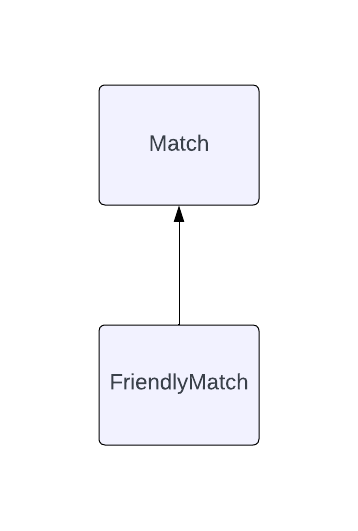
\includegraphics[width=0.3\linewidth]{MATCH.png}
        \caption{UML Match}
        \label{fig:enter-label}
    \end{figure}
     \item \textbf{PerformanceStats}

     Invece, in PerformanceStats sono state aggiunte due sottoclassi, disgiunte tra di loro, \textit{PlayerPerformanceStats}, e \textit{TeamPerformanceStats}. Questo è stato fatto per distinguere meglio il concetto di statistiche su un match, e statistiche di un singolo player.
     Per esempio la statistica del possesso palla non è concetto che è associato a un singolo calciatore ma è associata alla squadra.ù
     \begin{figure}[H]
         \centering
         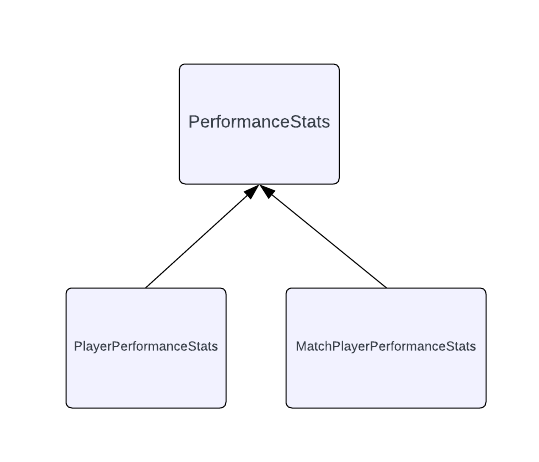
\includegraphics[width=0.4\linewidth]{STATS.png}
         \caption{UML PerformanceStats}
         \label{fig:enter-label}
     \end{figure}
     \item \textbf{Position}

      In Position, sono state definite le  specifiche posizioni in campo, così da rappresentare in modo preciso e strutturato il ruolo dei giocatori all'interno della formazione. Nell'ontologia originale erano modellate come Data Properties.
     \begin{figure}[H]
         \centering
         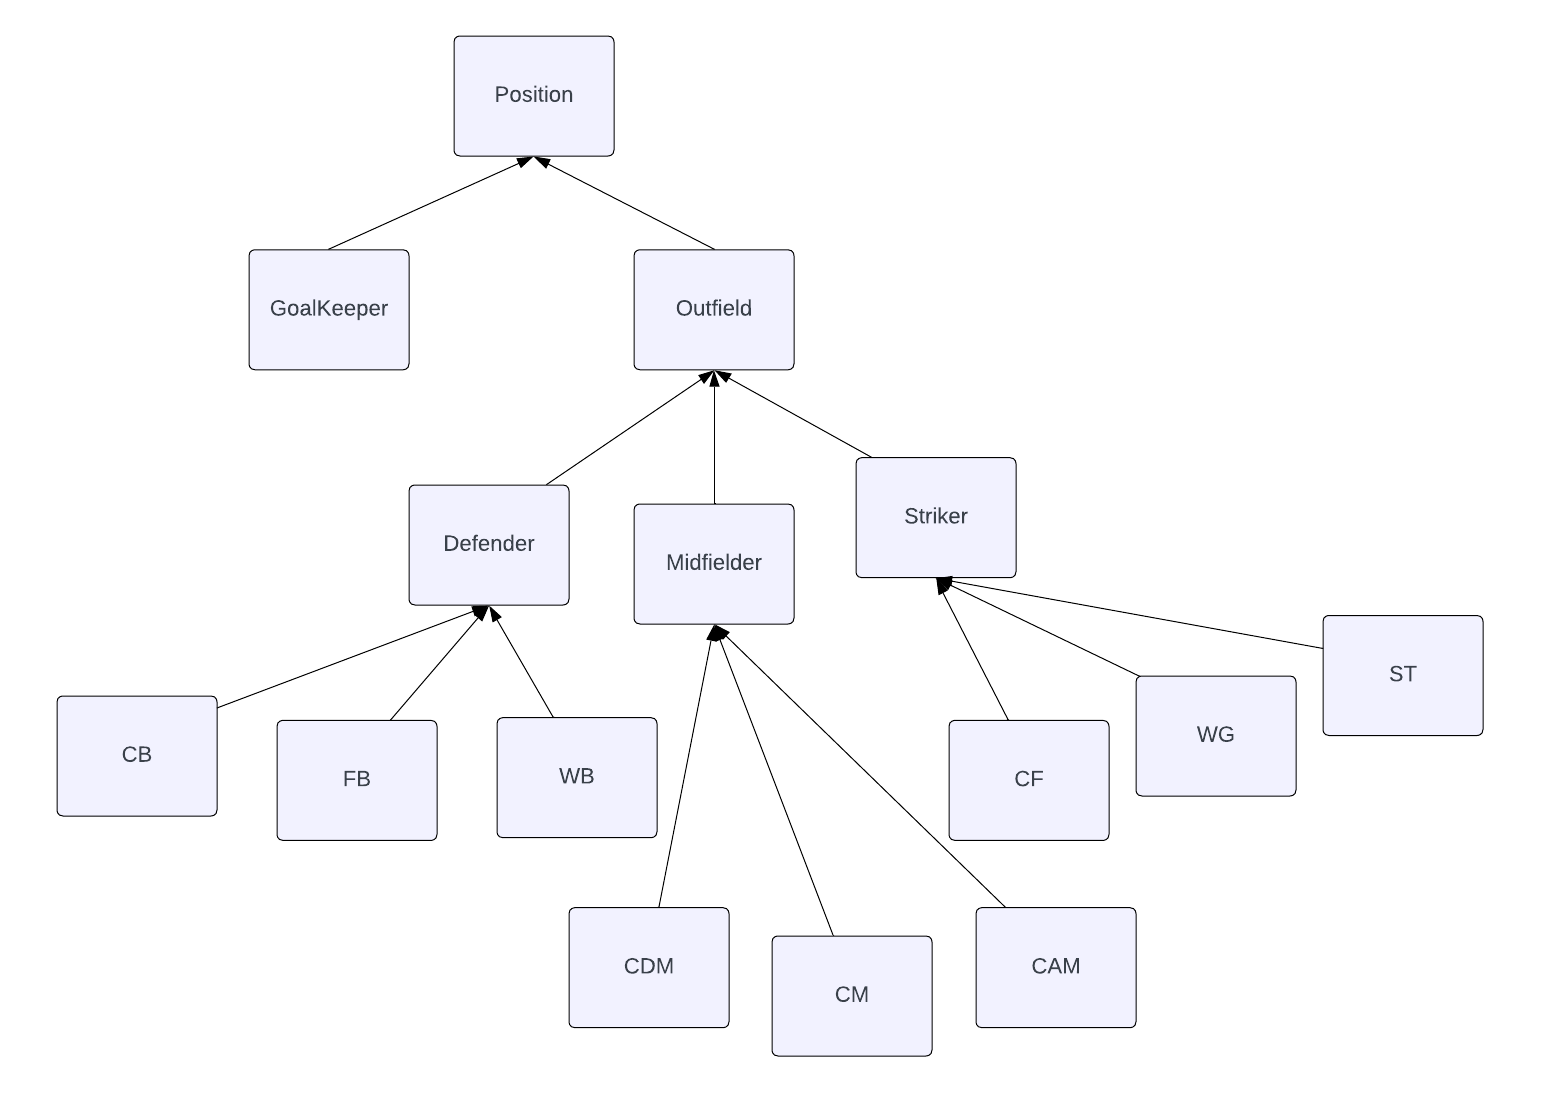
\includegraphics[width=1\linewidth]{POSITION.png}
         \caption{UML Position}
         \label{fig:enter-label}
     \end{figure}
    \hspace{2cm}

    Le abbreviazioni CB, FB, WB, CDM, etc indicano le specifiche posizioni in campo, per esempio CB significa Central Back, cioè Difensore centrale.

    \hspace{6cm}
     \item \textbf{Player}

     La classe Player infine è stata modificata in due classi equivalenti: CanBeCarded e ContractParticipant. Queste sono sottoclassi di Person; Person importata da \textit{schema.org}, vedi prossima sezione.
 \end{itemize}
\newpage

\section{Join con altre ontologie}

Come richiesto dalla consegna, è stato necessario integrare l'ontologia con altre ontologie esistenti, facendo operazioni di join per favorire l'interoperabilità dei concetti.

In particolare, sono stati importati:

\begin{itemize}
  \item La classe \textbf{Person} dall'ontologia \textit{schema.org}, utilizzata per rappresentare entità individuali come giocatori, illenatori e arbitri. 
  
  Nella nostra ontologia, \textit{Person} è stata inserita come superclasse delle classi \textit{Player}, \textit{Coach} e \textit{Referee}. Il join è stato eseguito in modo da includere solo le \textit{Object Properties} che ci interessavano, escludendo quelle non rilevanti  per il nostro dominio.

  \begin{figure}[H]
      \centering
      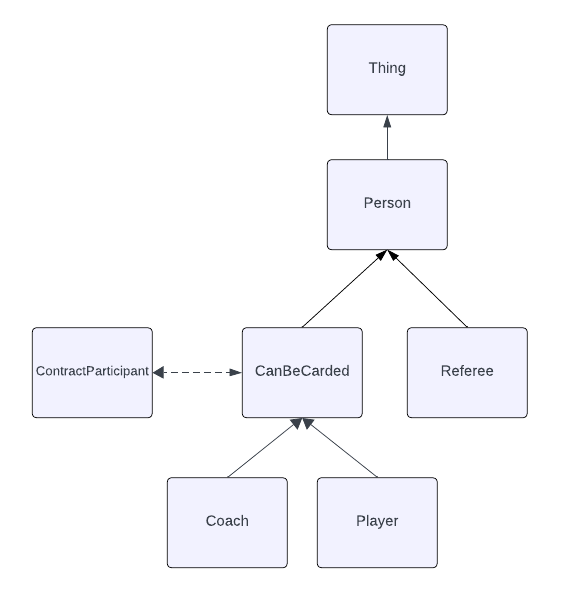
\includegraphics[width=0.7\linewidth]{PERSON.png}
      \caption{Enter Caption}
      \label{fig:enter-label}
  \end{figure}

  \item Le classi \textbf{City} e \textbf{Country} da \textit{dbpedia.org}, adottate per modellare i concetti geografici. 
  
  Anche in questo caso è stato effettuato un join selettivo: \textit{City} e \textit{Country} sono state collegate alla nostra ontologia per rappresentare, rispettivamente, la città dello stadio, la nazione della lega, e la nazionalità delle persone, attraverso la superclasse \textit{Person}.
\end{itemize}

\newpage


 \section{Classi aggiunte}

\begin{itemize}[leftmargin=*]
  \item \textbf{Contract}
  \begin{itemize}[leftmargin=2em]
    \item CoachContract
    \item PlayerContract
  \end{itemize}

  \item \textbf{Formation}
  \begin{itemize}[leftmargin=2em]
    \item 343
    \item 352
    \item 424
    \item 433
    \item 442
    \item 451
    \item 523
    \item 532
    \item 541
  \end{itemize}

  \item \textbf{MatchEvent}
  \begin{itemize}[leftmargin=2em]
    \item Card
    \begin{itemize}[leftmargin=2em]
      \item RedCard
      \item YellowCard
    \end{itemize}

    \item Corner

    \item FreeKick
    \begin{itemize}[leftmargin=2em]
      \item PenaltyKick
    \end{itemize}

    \item Goal
    \item Offside
    \item Substitution
  \end{itemize}

  \item \textbf{Season}
\end{itemize}




 \subsection{Classi d'errore}

 \newpage
 \section{Proprietà Aggiunge}

\chapter{Inserimento di individui}

\chapter{Regole SWRL}

\textbf{SWRL} (\textbf{Semantic Web Rule Language}) è un linguaggio usato nell'ambito del Semantic Web per esprimere regole di inferenza e vincoli logici più complessi di quelli realizzabili usando il solo OWL.

\hfill

Nella nostra ontologia abbiamo inserito numerose regole, utili a:

\begin{enumerate}
    \item inferire nuovi collegamenti tra i dati
    \item individuare casi di errore sui dati
\end{enumerate}

Le sezioni che seguono riportano tali regole, non in un ordine particolare.

\section{HomeFormationRule}

Questa regola "raffina" il collegamento tra una formazione e una partita, esplicitando che la prima è usata dalla squadra in casa.
Questo perché \texttt{isAwayFormationIn} è una sottoproprietà di \texttt{isFormationIn}.

\begin{lstlisting}[language=SWRL]
isHomeTeam(?t, ?m) ^ hasFormation(?t, ?f) ^ isFormationIn(?f, ?m) -> isHomeFormationIn(?f, ?m)
\end{lstlisting}

\section{AwayFormationRule}

Questa regola funziona in modo analogo alla precedente, ma riguardo la squadra in trasferta.

\begin{lstlisting}[language=SWRL]
isAwayTeam(?t, ?m) ^ hasFormation(?t, ?f) ^ isFormationIn(?f, ?m) -> isAwayFormationIn(?f, ?m)
\end{lstlisting}

\newpage

\section{DuplicateSubstituteRule}

Questa regola verifica se un giocatore segnato come riserva partecipa a multiple sostituzioni come giocatore entrante, e in tale caso gli assegna una classe di errore.

\begin{lstlisting}[language=SWRL]
hasReservePlayer(?f, ?p) ^ hasEnteringPlayer(?s1, ?p) ^ hasEnteringPlayer(?s2, ?p) ^ differentFrom(?s1, ?s2) ^ hasTeamFormation(?m, ?f) ^ hasSubstitution(?m, ?s1) ^ hasSubstitution(?m, ?s2) -> DuplicateSubstituteError(?p)
\end{lstlisting}

\section{DuplicateSubstitutedRule}

Il funzionamento di questa regola è analogo alla precedente, ma riguardante il giocatore uscente.
Questa regola copre però solo i giocatori titolari (ovvero i giocatori che partecipano alla partita dall'inizio).

\begin{lstlisting}[language=SWRL]
hasStarterPlayer(?f, ?p) ^ hasExitingPlayer(?s1, ?p) ^ hasExitingPlayer(?s2, ?p) ^ differentFrom(?s1, ?s2) ^ hasTeamFormation(?m, ?f) ^ hasSubstitution(?m, ?s1) ^ hasSubstitution(?m, ?s2) -> DuplicateSubstitutedError(?p)
\end{lstlisting}

\section{StarterAsSubstituteRule}

Questa regola verifica se un giocatore titolare è il giocatore entrante in una sostituzione, e in tale caso gli assegna una classe di errore.

\begin{lstlisting}[language=SWRL]
hasStarterPlayer(?f, ?p) ^ hasEnteringPlayer(?s, ?p) ^ hasTeamFormation(?m, ?t) ^ hasSubstitution(?m, ?s) -> StarterAsSubstituteError(?p)
\end{lstlisting}

\section{FriendlyMatchInTournamentRule}

Non è corretto assegnare una partita amichevole ad un torneo, qualsiasi sia il suo tipo, e se ciò viene fatto allora una classe di errore è assegnata alla partita. 

\begin{lstlisting}[language=SWRL]
includedInTournament(?m, ?t) ^ FriendlyMatch(?m) -> FriendlyMatchInTournamentError(?m)
\end{lstlisting}

\section{GoalScoredByTeamRule}

Questa regola collega un goal ad una squadra, sapendo che il goal è stato fatto da un giocatore che giocava in tale squadra nella partita.

\begin{lstlisting}[language=SWRL]
scores(?p, ?g) ^ hasEvent(?m, ?g) ^ isPlayerInFormation(?p, ?f) ^ hasFormation(?t, ?f) ^ competesIn(?t, ?m) -> scoredByTeam(?g, ?t)
\end{lstlisting}

\section{InconsistentBallPossessionInMatchRule}

Questa regola controlla se la somma del possesso palla indicata nelle statistiche di performance per le squadre che hanno giocato una partita non è 100\%, e in tale caso assegna una classe di errore alla partita e alle statistiche.

\begin{lstlisting}[language=SWRL]
teamStatsIn(?ps1, ?m) ^ teamStatsIn(?ps2, ?m) ^ differentFrom(?ps1, ?ps2) ^ BallPossession(?ps1, ?p1) ^ BallPossession(?ps2, ?p2) ^ swrlb:add(?r, ?p1, ?p2) ^ swrlb:notEqual(?r, 100) -> InconsistentBallPossessionInMatchError(?m) ^ InconsistentBallPossessionInMatchError(?ps1) ^ InconsistentBallPossessionInMatchError(?ps2)
\end{lstlisting}

\section{InconsistentContractDatesRule}

Questa regola verifica se le date di un contratto sono inconsistenti (data di inizio futura alla data di fine).

\begin{lstlisting}[language=SWRL]
ContractStartDate(?c, ?sd) ^ ContractEndDate(?c, ?ed) ^ temporal:before(?ed, ?sd) -> InconsistentContractDatesError(?c)
\end{lstlisting}

\section{InconsistentMatchScoresHome/AwayRule}

Queste due regole verificano se il vincitore di una partita non è consistente con i punteggi assegnati alle due squadre.
Sono state necessarie due regole in quanto i punteggi delle squadre sono legati alla partita e non direttamente alle squadre.

\begin{lstlisting}[language=SWRL]
isHomeTeam(?t1, ?m) ^ isAwayTeam(?t2, ?m) ^ hasWinner(?m, ?t1) ^ MatchHomeTeamScore(?m, ?s1) ^ MatchAwayTeamScore(?m, ?s2) ^ swrlb:lessThanOrEqual(?s1, ?s2) -> InconsistentMatchScoresError(?m)
\end{lstlisting}

\begin{lstlisting}[language=SWRL]
isHomeTeam(?t1, ?m) ^ isAwayTeam(?t2, ?m) ^ hasWinner(?m, ?t2) ^ MatchHomeTeamScore(?m, ?s1) ^ MatchAwayTeamScore(?m, ?s2) ^ swrlb:lessThanOrEqual(?s2, ?s1) -> InconsistentMatchScoresError(?m)
\end{lstlisting}

\section{InvalidLeagueMatchFormatExtraTime/PenaltyRule}

Le partite che fanno parte di una lega non possono avere supplementari o rigori, e queste due regole servono a identificare tali inconsistenze.

\begin{lstlisting}[language=SWRL]
includedInTournament(?m, ?t) ^ League(?t) ^ ExtraTimePlayed(?m, true) -> InvalidLeagueMatchFormatError(?m)
\end{lstlisting}

\begin{lstlisting}[language=SWRL]
includedInTournament(?m, ?t) ^ League(?t) ^ PenaltyShootoutPlayed(?m, true) -> InvalidLeagueMatchFormatError(?m)
\end{lstlisting}

\section{InvalidMatchRule}

Questa regola verifica se una squadra sta giocando contro sé stessa in una partita.

\begin{lstlisting}[language=SWRL]
hasHomeTeam(?m, ?t) ^ hasAwayTeam(?m, ?t) -> InvalidMatchError(?m)
\end{lstlisting}

\section{MultipleRedCardsRule}

Questa regola controlla se un giocatore ha ricevuto multipli cartellini rossi in una partita.

\begin{lstlisting}[language=SWRL]
hasReceived(?p, ?c1) ^ hasReceived(?p, ?c2) ^ RedCard(?c1) ^ RedCard(?c2) ^ differentFrom(?c1, ?c2) ^ hasEvent(?m, ?c1) ^ hasEvent(?m, ?c2) -> MultipleRedCardsError(?p)
\end{lstlisting}

\section{NonGoalKeeperWithSavesRule}

Questa regola verifica se le statistiche di un giocatore indicano il numero di parate sebbene esso non abbia giocato come portiere nella partita.

\begin{lstlisting}[language=SWRL]
playsInPosition(?pl, ?p) ^ Outfield(?p) ^ hasPlayerStats(?pl, ?ps) ^ Saves(?ps, ?s) ^ hasPlayer(?m, ?p) ^ hasPlayerPerformanceStats(?m, ?ps) -> NonGoalKeeperWithSavesError(?pl)
\end{lstlisting}

\section{PlayerInMatchRule}

Questa regola collega un giocatore ad una partita, sapendo che il giocatore era in una formazione utilizzata in tale partita.

\begin{lstlisting}[language=SWRL]
hasPlayerInFormation(?f, ?p) ^ isFormationIn(?f, ?m) -> hasPlayer(?m, ?p)
\end{lstlisting}

\section{TeamNotInMatchRule}

Questa regola controlla se un evento in una partita è legato ad una squadra che non gioca in tale partita.

\begin{lstlisting}[language=SWRL]
hasEvent(?m, ?e) ^ hasMatchEvent(?t, ?e) ^ isHomeTeam(?t1, ?m) ^ isAwayTeam(?t2, ?m) ^ differentFrom(?t, ?t1) ^ differentFrom(?t, ?t2) -> TeamNotInMatchError(?t)
\end{lstlisting}

\newpage

\section{UncontractedPlayerInMatchRule}

Questa regola verifica se un giocatore ha partecipato ad una partita senza far parte di una delle due squadre coinvolte, in quanto non si trovava sotto contratto con una delle due squadre al momento della partita.
La regola copre soltanto i casi in cui il giocatore si trovava sotto contratto con un'altra squadra e se il contratto è terminato.

\begin{lstlisting}[language=SWRL]
signs(?t1, ?c) ^ involvesPlayer(?c, ?p) ^ participatesIn(?p, ?m) ^ includes(?m, ?t2) ^ includes(?m, ?t3) ^ differentFrom(?t1, ?t2) ^ differentFrom(?t1, ?t3) ^ ContractStartDate(?c, ?sd) ^ ContractEndDate(?c, ?ed) ^ MatchDate(?m, ?d) ^ temporal:before(?sd, ?d) ^ temporal:after(?ed, ?d) -> UncontractedPlayerInMatchError(?p)
\end{lstlisting}

\chapter{Interrogazioni SPARQL}

L'ultima parte del progetto è stata la realizzazione di interrogazioni usando \textbf{SPARQL} (\textbf{SPARQL Protocol and RDF Query Language}), un linguaggio simile a SQL per poter estrarre dati dall'ontologia.

\hfill

Le interrogazioni che abbiamo scritto sono esempi che producono risultati sulla base degli individui d'esempio che abbiamo predisposto. 
Per realizzarle abbiamo usato le viste \textbf{SPARQL Query} e \textbf{Snap SPARQL Query} di Protegé. 

\section{Interrogazione sui contratti di un giocatore}

Questa interrogazione recupera i contratti firmati da un giocatore (nell'esempio \texttt{Player1}) e i nomi dei team per cui i contratti sono stati firmati. 

\begin{lstlisting}
PREFIX : <http://visualdataweb.org/FootOntologyPlus/>

SELECT ?contract ?teamName
WHERE { 
    ?team :signsPlayer ?contract ;
          :TeamName ?teamName .
    ?contract :involvesPlayer :Player1 .
}
\end{lstlisting}

\begin{figure}[H]
	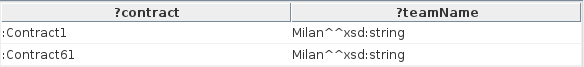
\includegraphics[width=\textwidth]{query1}
	\caption{Risultato della query sulla nostra ontologia.}
\end{figure}

\newpage

\section{Interrogazione sui contratti non terminati}

Questa interrogazione recupera tutti i contratti che non hanno una data di terminazione. Si assume in questo caso che tali contratti siano ancora attivi, ma in generale vige la "Open World assumption" riguardo alle informazioni mancanti.

\begin{lstlisting}
PREFIX : <http://visualdataweb.org/FootOntologyPlus/>

SELECT ?player ?team ?contract ?startDate
WHERE { 
    ?contract :isSignedForPlayerBy ?team ;
        :involvesPlayer ?player ;
        :ContractStartDate ?startDate .
    FILTER NOT EXISTS { ?contract :ContractEndDate ?endDate }
}
ORDER BY ASC (?player)
\end{lstlisting}

\begin{figure}[H]
	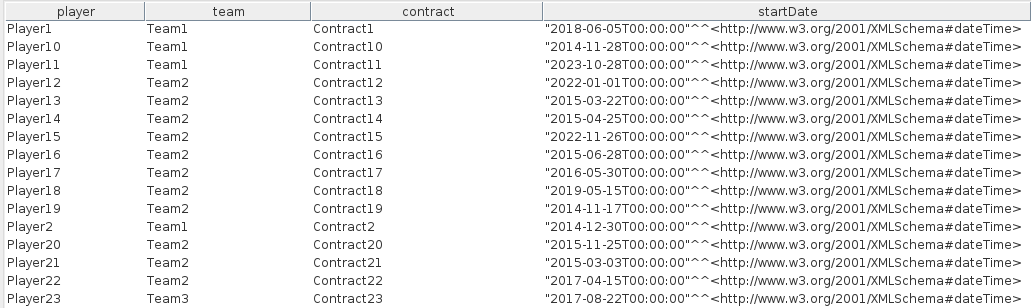
\includegraphics[width=\textwidth]{query2}
	\caption{Parte del risultato della query sulla nostra ontologia.}
\end{figure}

\section{Interrogazione sui cartellini ricevuti dai giocatori}

Questa interrogazione recupera le informazioni riguardanti i cartellini ricevuti dai giocatori, nello specifico il tipo di cartellino, la partita e il minuto di gioco in cui è stato ricevuto. 

\begin{lstlisting}
PREFIX rdf: <http://www.w3.org/1999/02/22-rdf-syntax-ns#>
PREFIX rdfs: <http://www.w3.org/2000/01/rdf-schema#>
PREFIX : <http://visualdataweb.org/FootOntologyPlus/>

SELECT ?player ?cardType ?match ?minute
WHERE {
    ?player :hasReceived ?card .
    ?card :MinuteOfEvent ?minute ;
        :isEventIn ?match ;
        rdf:type ?cardType .
    ?cardType rdfs:subClassOf :Card .
    FILTER (?cardType != :Card) .
}
ORDER BY ASC (?player)
\end{lstlisting}

\begin{figure}[H]
	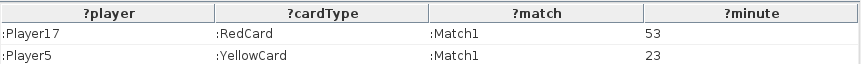
\includegraphics[width=\textwidth]{query3}
	\caption{Risultato della query sulla nostra ontologia.}
\end{figure}

\section{Interrogazione sulle sostituzioni effettuate in una partita}

Questa interrogazione le informazioni riguardanti le sostituzioni effettuate in una partita (nell'esempio \texttt{Match1}), nello specifico il nome dei giocatori coinvolti e il minuto di gioco. 

\begin{lstlisting}
PREFIX : <http://visualdataweb.org/FootOntologyPlus/>

SELECT ?enteringName ?exitingName ?minute
WHERE {
    ?sub :isSubstitutionIn :Match1 ;
        :hasEnteringPlayer ?entering ;
        :hasExitingPlayer ?exiting ;
        :MinuteOfEvent ?minute .
    ?entering :FullName ?enteringName .
    ?exiting :FullName ?exitingName .
}
ORDER BY ASC (?minute)
\end{lstlisting}

\begin{figure}[H]
	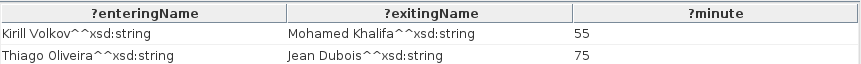
\includegraphics[width=\textwidth]{query4}
	\caption{Risultato della query sulla nostra ontologia.}
\end{figure}

\section{Interrogazione sui goal segnati dai giocatori}

Questa interrogazione recupera il numero di goal segnati da ogni giocatore in un torneo (nell'esemptio \texttt{League1}).

\begin{lstlisting}
PREFIX : <http://visualdataweb.org/FootOntologyPlus/>

SELECT ?player ?playerName (COUNT(?goal) as ?totalGoals) 
WHERE {
    ?match :includedInTournament :League1 ;
        :hasGoal ?goal .
    ?goal :scoredByPlayer ?player .
    ?player :FullName ?playerName
}
GROUP BY ?player ?playerName
ORDER BY DESC (?totalGoals)
\end{lstlisting}

\begin{figure}[H]
	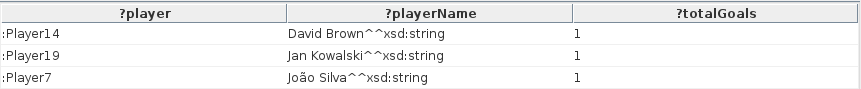
\includegraphics[width=\textwidth]{query5}
	\caption{Risultato della query sulla nostra ontologia. Il nome dell'individuo giocatore è incluso in caso di omonimi.}
\end{figure}



\chapter{Conclusioni}

\medspace

\printbibliography

\end{document}
